\section{Grundlagen}


\subsection{Anwendungsdomäne}

Der resultierende Prototyp kann auf Baustellen eingesetzt werden, um die Anschlagspunkte verschiedener Lasten automatisch zu erkennen. Dies umfasst typischerweise Lasten wie Betonelemente, Stahlträger und Holzkonstruktionen. Die Umgebungsbedingungen auf Baustellen, wie variable Wetterbedingungen und begrenzter Platz, stellen besondere Anforderungen an die Robustheit und Genauigkeit der Kameratechnik und Software. Baustellenarbeiter interagieren über eine benutzerfreundliche Schnittstelle mit dem System, das ihre Arbeit durch erhöhte Sicherheit und Effizienz unterstützt.


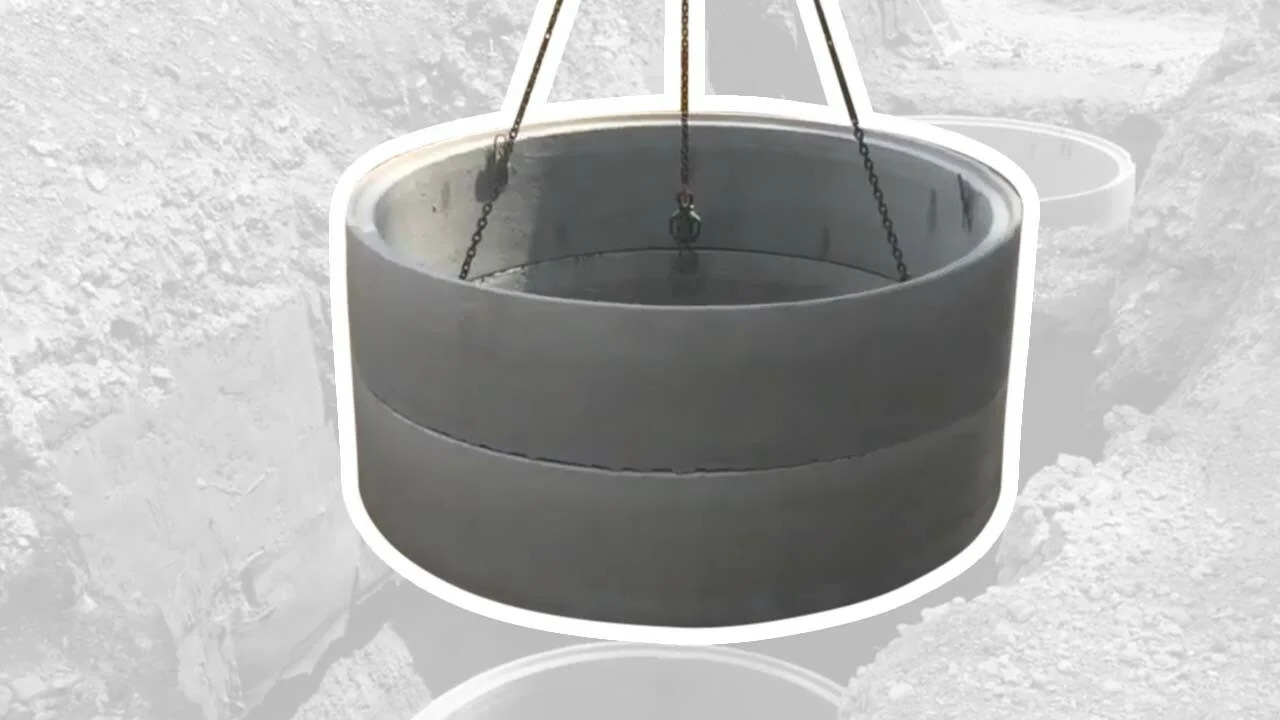
\includegraphics[width=0.5\textwidth]{graphics/Betonelement.jpg}\hfill%
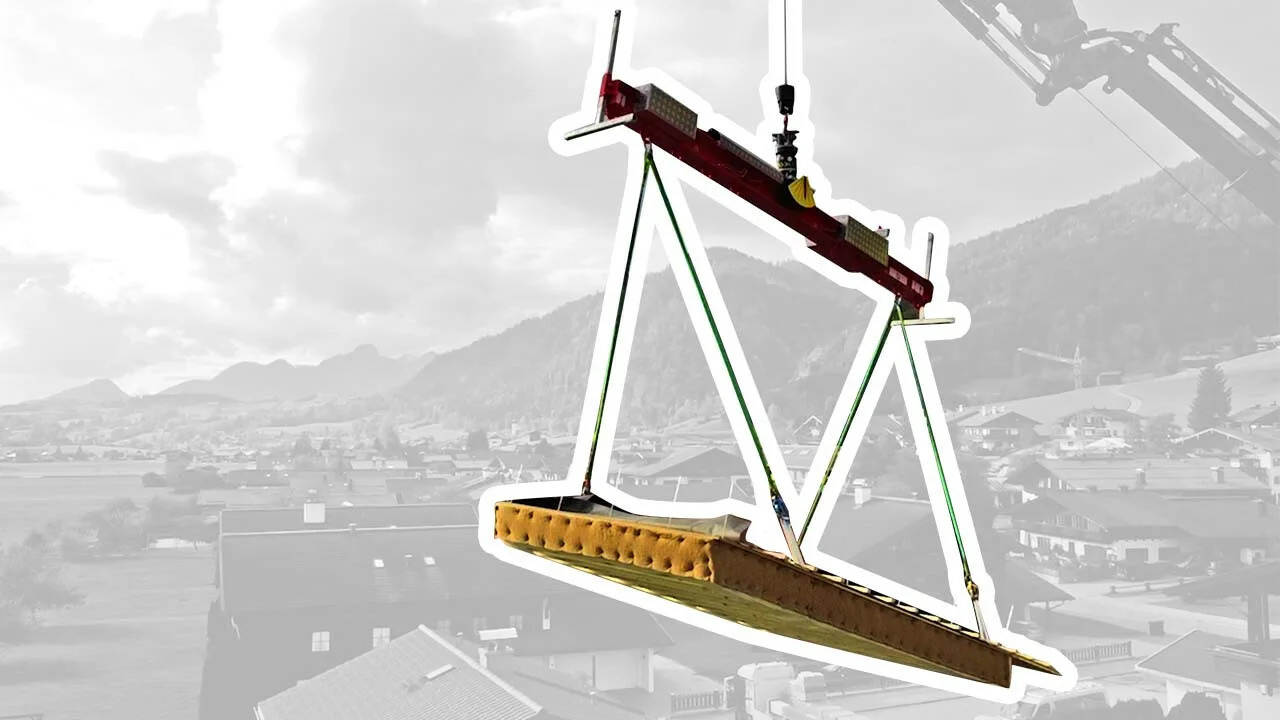
\includegraphics[width=0.5\textwidth]{graphics/Traverse.jpg}



\subsection{Traverse}
Die Traverse hat eine Dimension(Länge X Breite X Höhe) von 500cm X 70cm X 50cm.

\begin{figure}[h]
    \centering
    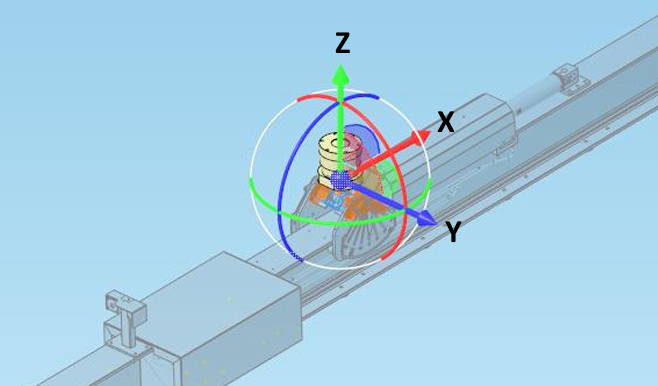
\includegraphics[width=0.5\linewidth]{graphics/Traverse_Rotationen.PNG}
    \caption{Koordinaten-System der Ludwig System Traverse}
    \label{fig:traverse}
\end{figure}

Abbildung \ref{fig:traverse} zeigt das linkshändige Koordinaten-System der Traverse. Dabei wird fortan die Rotation um die Y-Achse der Traverse als Neigen definiert und die Rotation um die Z-Achse der Traverse, als Rotieren definiert.

\subsection{Last}
Unter Lasten sind vor allem Fertigstrukturen wie z.B. Fertig erstellte Wände oder Dächer. Lasten haben maximal 2 Anschlagspunkte, welche einen Abstand von 1m bis 6m zueinander haben. Diese Anschlagspunkte können auf unterschiedliche Höchen sein, wie z.B. bei Dächer welche eine Neigung besitzen.


\subsection{Stand der Forschung}

\subsubsection{Arbeit: Objekterkennung und Distanzmessung für KollisionsVermeidung bei Lastenhebung}
(Arbeit: Object Detection and Distance Measurement Algorithm for Collision Avoidance of Precast Concrete Installation during Crane Lifting Process\cite{yong_object_2023} Erklären)

\subsubsection{Arbeit: Objekterkennung und 3D-basierte Objektortung für automatische Lastenhebung}
(Arbeit: Image-based onsite object recognition for automatic crane lifting tasks\cite{zhou_image-based_2021} Erklären)





